\documentclass{article}
\pagestyle{empty}

%% >>> preamble
\usepackage{pgfplots}
\pgfplotsset{compat=1.18}
%% <<< preamble

\begin{document}
%% >>> snippet
\begin{figure}[htbp]
  \centering
  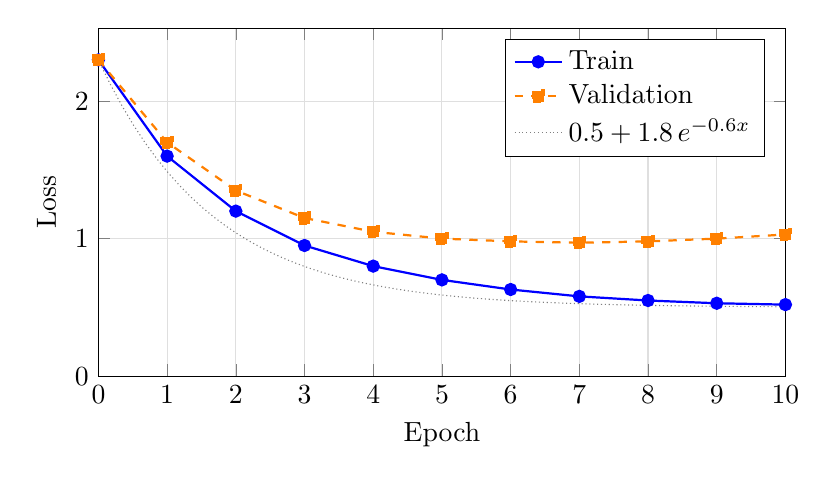
\begin{tikzpicture}
    \begin{axis}[
        width=0.85\textwidth, height=6cm,
        xlabel={Epoch}, ylabel={Loss},
        xmin=0, xmax=10, ymin=0,
        grid=major, grid style={gray!25},
        legend pos=north east, legend cell align=left,
      ]
      \addplot[thick, blue, mark=*] coordinates {
        (0,2.30) (1,1.60) (2,1.20) (3,0.95) (4,0.80) (5,0.70)
        (6,0.63) (7,0.58) (8,0.55) (9,0.53) (10,0.52)};
      \addlegendentry{Train}
      \addplot[thick, orange, dashed, mark=square*] coordinates {
        (0,2.30) (1,1.70) (2,1.35) (3,1.15) (4,1.05) (5,1.00)
        (6,0.98) (7,0.97) (8,0.98) (9,1.00) (10,1.03)};
      \addlegendentry{Validation}
      \addplot[gray, densely dotted, domain=0:10, samples=60] {0.5 + 1.8*exp(-0.6*x)};
      \addlegendentry{$0.5 + 1.8\,e^{-0.6x}$}
    \end{axis}
  \end{tikzpicture}
  \caption{Training curves drawn with \texttt{pgfplots}.}
  \label{fig:loss}
\end{figure}
%% <<< snippet
\end{document}
